\documentclass[convert={density=300,outext=.png}]{standalone}
\usepackage{tikz}
\usetikzlibrary{shapes,arrows,decorations,decorations.pathmorphing,arrows.meta,patterns,decorations.markings}

\begin{document}
%% Use \usepackage{tikz}
%% Use \usetikzlibrary{shapes,arrows,decorations, decorations.pathmorphing,arrows.meta,patterns}
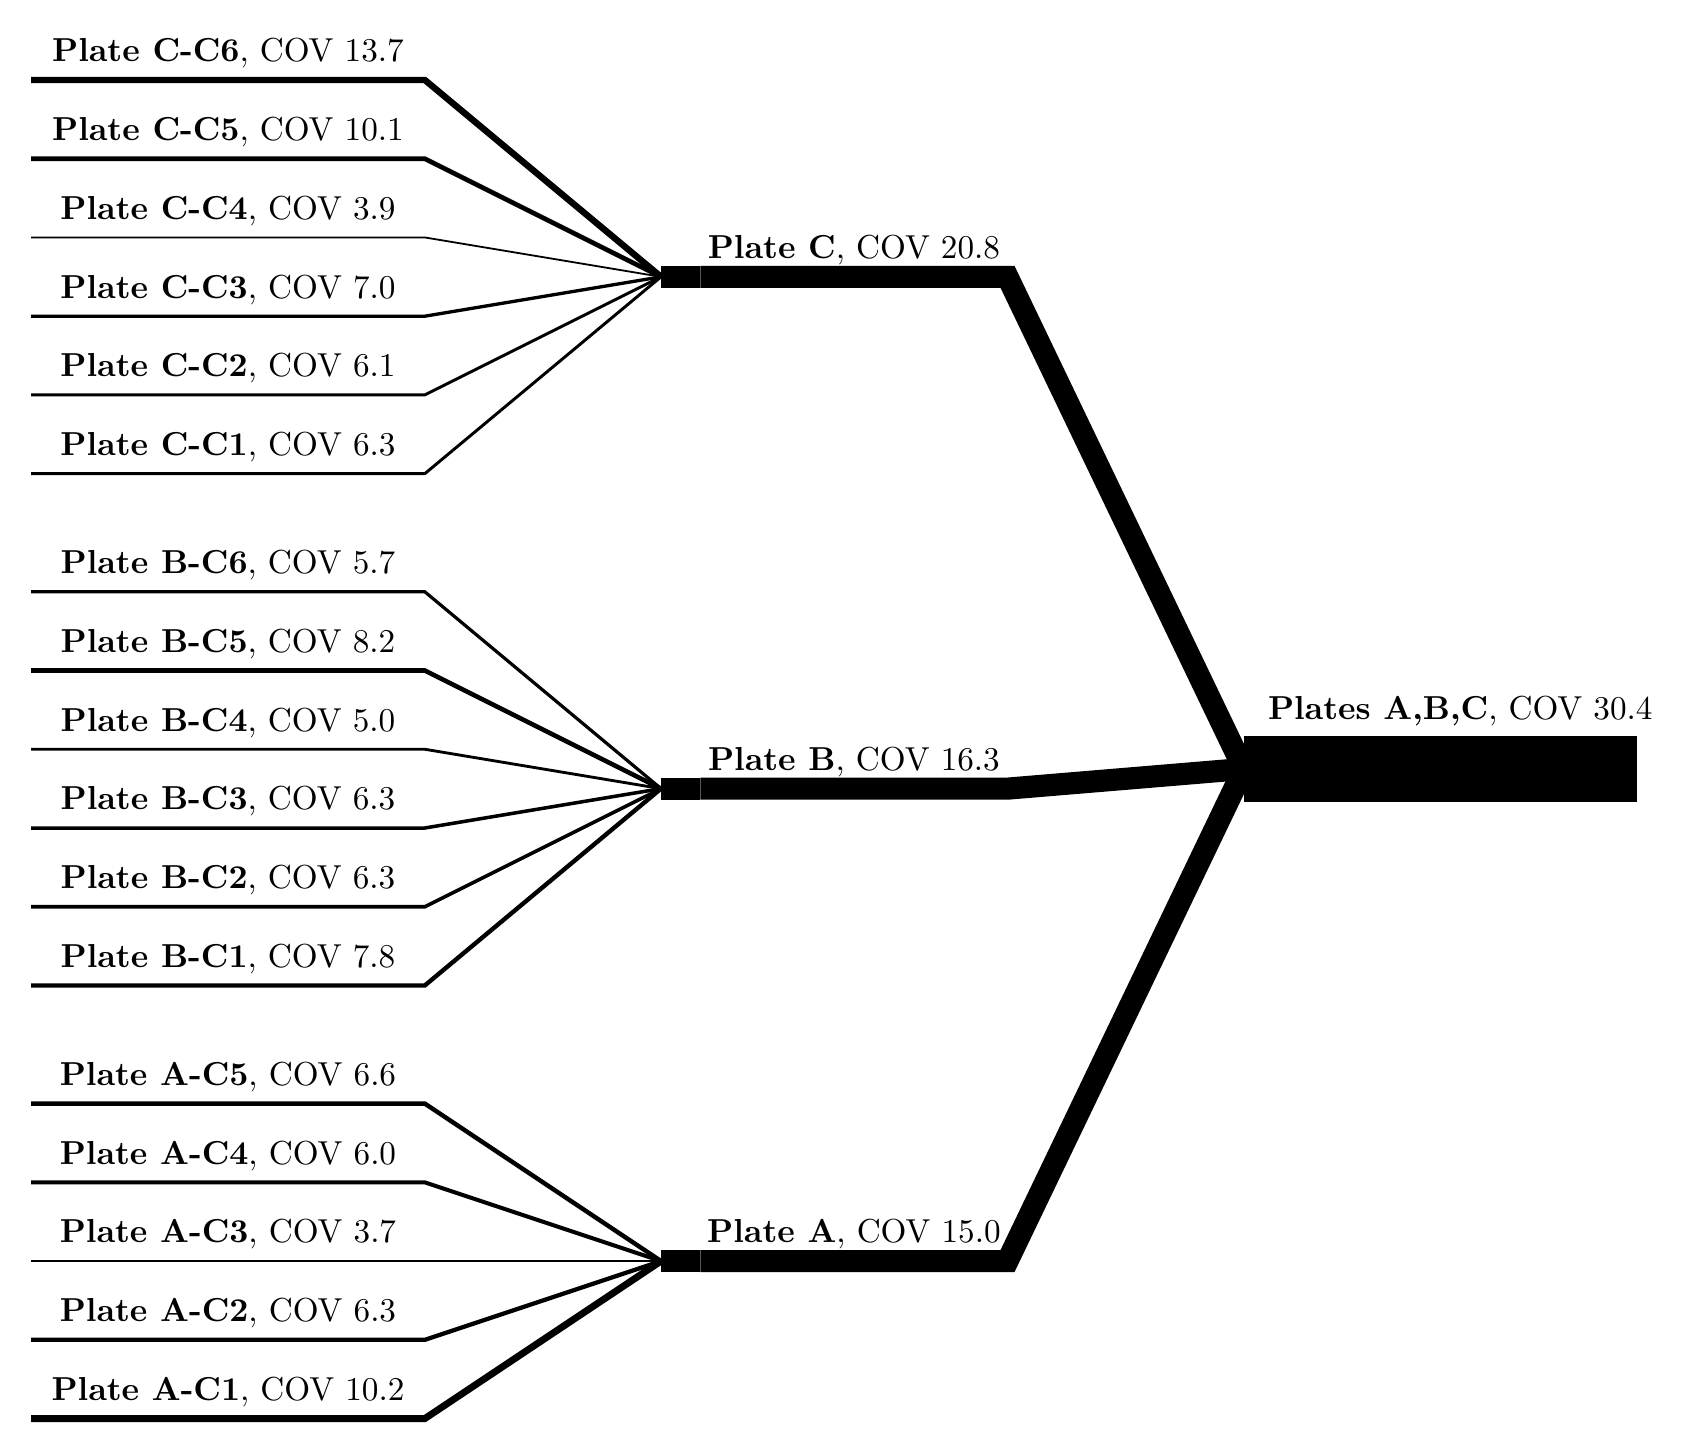
\begin{tikzpicture}[scale=1.0000]
	\tikzstyle{every node}=[scale=1.2000]
	
	%%Created with tikzpy
	
	\draw [line width = 24.0000]  (15.9000,8.2500,0.0000) -- (20.4000,8.2500,0.0000);
	\node [above ,align=left]  at (18.1500,8.6500,0.0000)  {\textbf{Plates A,B,C}, COV 30.4};
	\draw [line width = 2.4879]  (0.0000,0.0000,0.0000) -- (5.0000,0.0000,0.0000) -- (8.0000,2.0000,0.0000);
	\node [above ,align=left]  at (2.5000,0.0000,0.0000)  {\textbf{Plate A-C1}, COV 10.2};
	\draw [line width = 1.5342]  (0.0000,1.0000,0.0000) -- (5.0000,1.0000,0.0000) -- (8.0000,2.0000,0.0000);
	\node [above ,align=left]  at (2.5000,1.0000,0.0000)  {\textbf{Plate A-C2}, COV 6.3};
	\draw [line width = 0.8951]  (0.0000,2.0000,0.0000) -- (5.0000,2.0000,0.0000) -- (8.0000,2.0000,0.0000);
	\node [above ,align=left]  at (2.5000,2.0000,0.0000)  {\textbf{Plate A-C3}, COV 3.7};
	\draw [line width = 1.4694]  (0.0000,3.0000,0.0000) -- (5.0000,3.0000,0.0000) -- (8.0000,2.0000,0.0000);
	\node [above ,align=left]  at (2.5000,3.0000,0.0000)  {\textbf{Plate A-C4}, COV 6.0};
	\draw [line width = 1.6134]  (0.0000,4.0000,0.0000) -- (5.0000,4.0000,0.0000) -- (8.0000,2.0000,0.0000);
	\node [above ,align=left]  at (2.5000,4.0000,0.0000)  {\textbf{Plate A-C5}, COV 6.6};
	\draw [line width = 8.0000]  (8.0000,2.0000,0.0000) -- (8.5000,2.0000,0.0000);
	\draw [line width = 1.5838]  (0.0000,5.5000,0.0000) -- (5.0000,5.5000,0.0000) -- (8.0000,8.0000,0.0000);
	\node [above ,align=left]  at (2.5000,5.5000,0.0000)  {\textbf{Plate B-C1}, COV 7.8};
	\draw [line width = 1.2878]  (0.0000,6.5000,0.0000) -- (5.0000,6.5000,0.0000) -- (8.0000,8.0000,0.0000);
	\node [above ,align=left]  at (2.5000,6.5000,0.0000)  {\textbf{Plate B-C2}, COV 6.3};
	\draw [line width = 1.2745]  (0.0000,7.5000,0.0000) -- (5.0000,7.5000,0.0000) -- (8.0000,8.0000,0.0000);
	\node [above ,align=left]  at (2.5000,7.5000,0.0000)  {\textbf{Plate B-C3}, COV 6.3};
	\draw [line width = 1.0229]  (0.0000,8.5000,0.0000) -- (5.0000,8.5000,0.0000) -- (8.0000,8.0000,0.0000);
	\node [above ,align=left]  at (2.5000,8.5000,0.0000)  {\textbf{Plate B-C4}, COV 5.0};
	\draw [line width = 1.6648]  (0.0000,9.5000,0.0000) -- (5.0000,9.5000,0.0000) -- (8.0000,8.0000,0.0000);
	\node [above ,align=left]  at (2.5000,9.5000,0.0000)  {\textbf{Plate B-C5}, COV 8.2};
	\draw [line width = 1.1662]  (0.0000,10.5000,0.0000) -- (5.0000,10.5000,0.0000) -- (8.0000,8.0000,0.0000);
	\node [above ,align=left]  at (2.5000,10.5000,0.0000)  {\textbf{Plate B-C6}, COV 5.7};
	\draw [line width = 8.0000]  (8.0000,8.0000,0.0000) -- (8.5000,8.0000,0.0000);
	\draw [line width = 1.0657]  (0.0000,12.0000,0.0000) -- (5.0000,12.0000,0.0000) -- (8.0000,14.5000,0.0000);
	\node [above ,align=left]  at (2.5000,12.0000,0.0000)  {\textbf{Plate C-C1}, COV 6.3};
	\draw [line width = 1.0421]  (0.0000,13.0000,0.0000) -- (5.0000,13.0000,0.0000) -- (8.0000,14.5000,0.0000);
	\node [above ,align=left]  at (2.5000,13.0000,0.0000)  {\textbf{Plate C-C2}, COV 6.1};
	\draw [line width = 1.1918]  (0.0000,14.0000,0.0000) -- (5.0000,14.0000,0.0000) -- (8.0000,14.5000,0.0000);
	\node [above ,align=left]  at (2.5000,14.0000,0.0000)  {\textbf{Plate C-C3}, COV 7.0};
	\draw [line width = 0.6612]  (0.0000,15.0000,0.0000) -- (5.0000,15.0000,0.0000) -- (8.0000,14.5000,0.0000);
	\node [above ,align=left]  at (2.5000,15.0000,0.0000)  {\textbf{Plate C-C4}, COV 3.9};
	\draw [line width = 1.7143]  (0.0000,16.0000,0.0000) -- (5.0000,16.0000,0.0000) -- (8.0000,14.5000,0.0000);
	\node [above ,align=left]  at (2.5000,16.0000,0.0000)  {\textbf{Plate C-C5}, COV 10.1};
	\draw [line width = 2.3249]  (0.0000,17.0000,0.0000) -- (5.0000,17.0000,0.0000) -- (8.0000,14.5000,0.0000);
	\node [above ,align=left]  at (2.5000,17.0000,0.0000)  {\textbf{Plate C-C6}, COV 13.7};
	\draw [line width = 8.0000]  (8.0000,14.5000,0.0000) -- (8.5000,14.5000,0.0000);
	\draw [line width = 8.0000]  (8.5000,2.0000,0.0000) -- (12.4000,2.0000,0.0000) -- (15.4000,8.2500,0.0000);
	\node [above ,align=left]  at (10.4500,2.0000,0.0000)  {\textbf{\textbf{Plate A}}, COV 15.0};
	\draw [line width = 8.0000]  (8.5000,8.0000,0.0000) -- (12.4000,8.0000,0.0000) -- (15.4000,8.2500,0.0000);
	\node [above ,align=left]  at (10.4500,8.0000,0.0000)  {\textbf{\textbf{Plate B}}, COV 16.3};
	\draw [line width = 8.0000]  (8.5000,14.5000,0.0000) -- (12.4000,14.5000,0.0000) -- (15.4000,8.2500,0.0000);
	\node [above ,align=left]  at (10.4500,14.5000,0.0000)  {\textbf{\textbf{Plate C}}, COV 20.8};
	\draw [line width = 24.0000]  (15.4000,8.2500,0.0000) -- (15.9000,8.2500,0.0000);

\end{tikzpicture}
\end{document}
